\problemname{Bikes vs Cars}
In Lund, biking is a very common method of transportation. But it is sometimes difficult to 
fit both cars and cyclists on the narrow streets.
To improve the situation, the local governor wants to completely redesign the local street network. 

There are $N$ important locations (numbered from $0$ to $N-1$) in Lund that people frequently travel between.
People travel between two locations by following a path, which is a sequence of streets going from the first location to the other.
A vehicle (car or bike) can travel on a path if all relevant lanes are at least as wide as the vehicle.
Each newly built street connects two of these important locations and it has a total width of $W$.
This width can be arbitrarily partitioned between bike lane and car lane.
In Lund, some engineers have recently invented cars and bikes of width $0$ (these can travel on lanes with width $0$).

The engineers have measured the widths of the cars and bikes in the city. 
For each pair of important locations, they know the widest car and the widest bike that should be able to travel between them, 
but the governor also requires that no wider cars or bikes can travel between these two locations.

Formally, you are given for each pair $i,j$ ($0 \le i<j \le N-1$) two integer values
$C_{i,j}$ and $B_{i,j}$. Your task is to construct a network of streets connecting the $N$ locations.
The streets all have a width of $W$, but for each street $s$ you can decide the
width of its bike lane $b_s$ and this determines the width of its car lane $W-b_s$.
The network must satisfy the following:

\begin{itemize}
  \item It is possible to travel between each pair of locations. Note that this might require a bike or car of width $0$.

  \item For each pair of locations $i$, $j$ (where $i < j$), it is possible to travel between 
  $i$ and $j$ by only using streets whose car lanes have a width of at least $C_{i,j}$. Also, $C_{i,j}$ is the 
  maximum number with this property. That is, for all paths between locations
    $i$ and $j$ it holds that at least one of the streets has a car lane of
    width at most $C_{i,j}$.

  \item For each pair of locations $i$, $j$ (where $i < j$), it is possible to travel between 
  $i$ and $j$ by only using streets whose bike lanes have a width of at least $B_{i,j}$. Also, $B_{i,j}$ is the 
  maximum number with this property.

\end{itemize}

Can you help the governor of Lund to design such a street network? 
Because the funding is limited, you can build at most $2023$ streets.
You can build multiple streets between the same pair of important locations but you cannot connect a location with itself.
All streets can be used in both directions.

\section*{Input}
The first line of input contains two integer $N$ and $W$, the number of important locations in Lund and the width of the streets that you can build.

The following $N-1$ lines contain the integers $C_{i,j}$. The $j$th of these lines will contain every
$C_{i,j}$ where $i < j$. So the first line will contain only $C_{0,1}$, the second will contain $C_{0,2}$
and $C_{1,2}$, the third $C_{0,3}$, $C_{1,3}$, $C_{2,3}$, and so on.

The following $N-1$ lines contain the integers $B_{i,j}$, on the same format as
$C_{i,j}$.

\section*{Output}

If it is impossible to construct such a street network, print one line with the string ``NO''.

Otherwise, print one line with the integer $M$, the number of streets of
your network.

For each of the following $M$ lines, print three integers $u, v, b$, indicating
that a street with a bike lane of width $b$ (and a car lane with width $W-b$) goes between $u$ and $v$.

You may use at most $2023$ streets. The streets you output must satisfy $0 \leq b \leq W$, $0\le u,v \le N-1$ and $u\neq v$. 
You may use multiple streets (possibly of different bike lane width) between the same pair of important locations.

In case there are multiple solutions, you may output any of them.

\section*{Constraints and Scoring}

\begin{itemize}
  \item $2 \le N \le 500$.
  \item $1 \le W \le 10^6$.
  \item $0 \le C_{i,j},B_{i,j}\le W$ for all $0 \le i < j \le N-1$.
\end{itemize}

\noindent
Your solution will be tested on a set of test groups, each worth a number of points. 
Each test group contains a set of test cases. To get the points for a test group you need to 
solve all test cases in the test group.

\noindent
\begin{tabular}{| l | l | p{12cm} |}
  \hline
  Group & Score & Constraints \\ \hline
  $1$   & $10$      & All $C_{i,j}$ are the same, and all $B_{i,j}$ are the same, $N \leq 40$.\\ \hline
  $2$   & $5$       & All $C_{i,j}$ are the same, and all $B_{i,j}$ are the same.\\ \hline
  $3$   & $17$      & $N\le 40$.\\ \hline
  $4$   & $18$      & $W = 1$.\\ \hline
  $5$   & $19$      & All $B_{i,j}$ are the same. \\ \hline
  $6$   & $31$      & No further constraints.  \\ \hline

\end{tabular}

\section*{Example}

In the first sample, the width of a street is $1$ and we need a car lane and a bike lane of width at least $1$ between locations $0$ and $1$. 
The solution is to have two separate streets connecting the locations, one with a bike lane of width $1$ and one with a car lane or width $1$.

\begin{figure}[h]
  \centering
  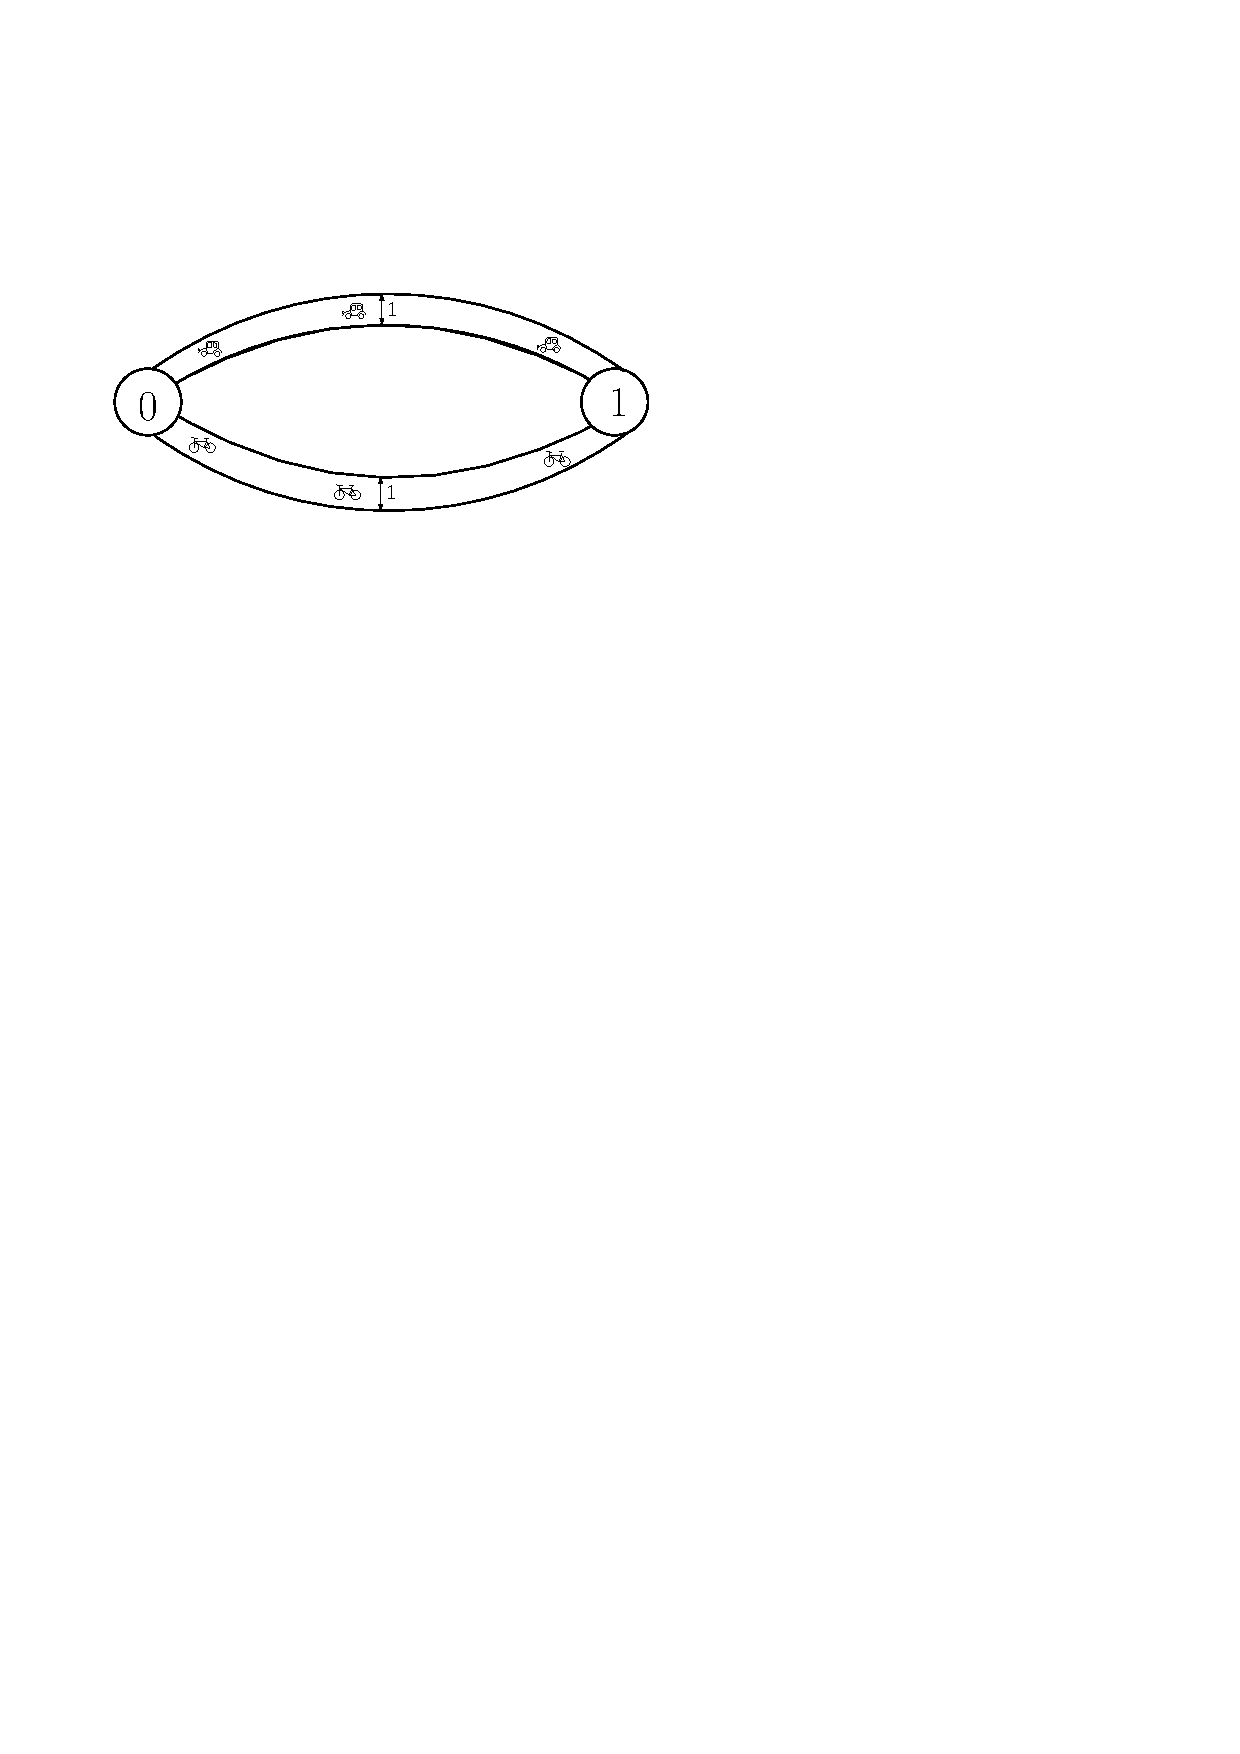
\includegraphics[width=.8\textwidth]{sample_small.pdf}
\end{figure}

In the second sample, the width of a street is again $1$ and there should be
a path with a bike lane of width $1$ between every pair
of important locations and there is a path between the locations $1$ and $2$ and $2$
and $3$ where the width of the car lane is $1$ for every street. This
contradicts the fact that, as $C_{1,3}=0$, there should not be a path with car lane width $1$
from  $1$ to $3$ as we can just join the two aforementioned paths to form such
a path. Thus it is not possible to construct such a street network.

In the third sample, the street network below fulfills all the conditions.
For example, there should be a path with minimum width of the car lane $1 = C_{0,5}$ 
between location $0$ and location $5$ (e.g.~by following the route $0\to 2\to 4 \to 5)$, 
a path where the bike lane has minimum width $3 = B_{0,5}$ (e.g.~by following the route $0\to 3 \to 4 \to 5)$. 
At the same time it can be checked that there are no paths with a wider minimum width for any of the connections. 
Note that there are many other solutions to the third sample.
\begin{figure}[h]
  \centering
  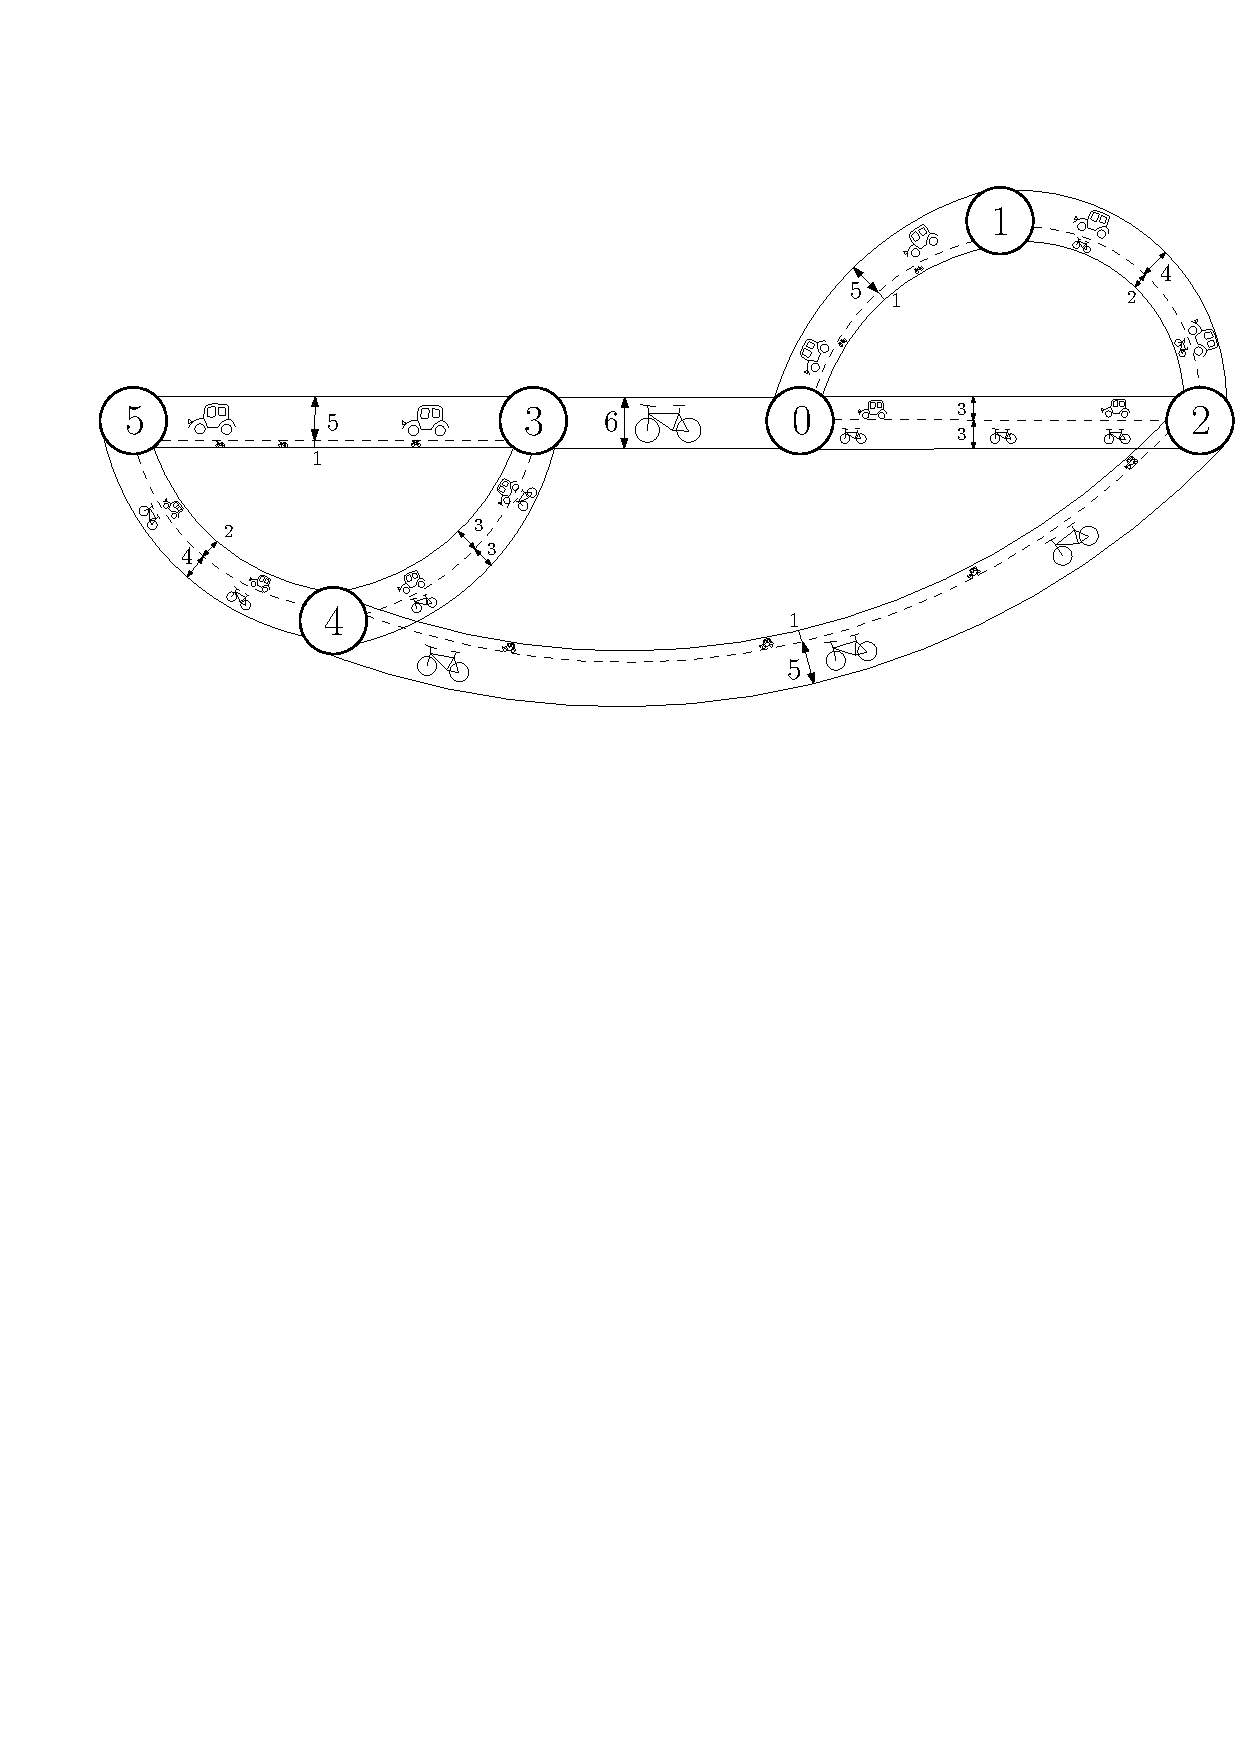
\includegraphics[width=.95\textwidth]{sample.pdf}
\end{figure}
